\chapter{可控核聚变的现况}
\section{国际热核聚变实验堆}
国际热核聚变实验反应堆是国际核聚变研究和巨型工程,这是目前正在建设世界上最大的实验性托卡马克核聚变反应堆,$ITER$将使用环形加速器产生温度超过$10$亿度的氢等离子体,它将产生大约$500MW$的核聚变能量,维持大约500秒;相比较而言欧洲联合环形加速器的最高纪录不过是$16MW$维持了不到1秒。作为聚变能实验堆,$ITER$要把上亿度、由氘氚组成的高温等离子体约束在体积$837m^{3}$的"磁笼"中,产生5亿瓦的聚变功率,持续时间达$500$秒。这是人类第一次获得接近电站规模的受控聚变能。


在$ITER$上开展的研究工作将揭示这种带有氘氚核聚变反应的高温等离子体的特性,探索它的约束、加热和能量损失机制,等离子体边界的行为以及最佳的控制条件,从而能够为今后建设商用的核聚变反应堆奠定坚实的科学基础。对$ITER$装置工程整体及各部件在5亿瓦聚变功率长时间持续过程中产生的变化及可能出现问题的研究,不仅将验证受控热核聚变能的工程可行性,而且还将对今后如何设计和建造聚变反应堆提供必不可少的信息。


同时值得说明的是,我国于2006年正式加入$ITER$计划,这显示了我国作为一个大国所应该有的国际担当,也显示了我国在科技领域也在逐步推行着改革开放的步伐,带动了我国不仅是核聚变领域,同时也有材料技术,激光技术以及超导技术等方面技术的提高,培养了一堆可靠的科研人才,推动了我国在科研领域的进展。
\section{中国“人造太阳”}
$EAST$是我国新时代“人造太阳”实验装置,位于中国合肥。2009年,$EAST$首轮物理放电实验取得成功,标志着我国站在了世界核聚变研究的前端。2012年4月19日,$EAST$中性束注入系统完成了氢离子束功率3兆瓦、脉冲宽度500毫秒的高能量离子束引出实验,这标志着我国自行研制的具有国际先进水平的中性束注入系统基本克服所有重大技术难关。2016年2月,$EAST$物理实验获重大突破,实现在国际上电子温度达到5000万度持续时间最长的等离子体放电。2018年,$EAST$实现1亿摄氏度等离子体运行等多项重大突破\cite{chinaEAST2}。


$EAST$相继完成了辅助加热、钨偏滤器、等离子体物理诊断等系统的升级改造,基本解决了射频波耦合、高约束等离子体稳定性控制、等离子体与壁相互作用物理、低动量条件下加热和电流驱动下输运、杂质输运和控制等问题,为实现长脉冲稳态高约束模等离子体奠定了基础,其稳态运行模式将为$ITER$和未来反应堆提供重要参考\cite{chinaEAST1}。


总的来说,我国的核科学研究虽然相较于国外起步晚,但是在我国科学家的不懈努力下,我们已经迎难而上,几乎走在了世界的前列,相信在不久后的将来我们也能够享受到核聚变能量带来的便利条件和发展了。
\section{核聚变能发展的必要性}
正如之前在背景中所描述的那样,对能源供应和消费的估计表明,本世纪中叶将是世界能源供应无法跟上需求的临界点。由于世界人口的增长和人均能源消费的增长,需求不可避免地增长;而技术经济进步与人均能源消耗密切相关。因此,能源供应不足将限制人类文明的进步,但是当核聚变技术完善到聚变燃烧氘时,即使能源消耗像过去一样持续增长,其燃料供应也将持续数百万年。而仅仅到了下个世纪,核聚变能源就应该能够填补这一空白,人类文明也能继续进步和增长。另一方面,如果没有核聚变能源,人类的命运将不可避免地严重衰退,世界人口将减少到50亿以下,最终甚至更低。如下图所示\cite{Lee2011NuclearFE}:
\begin{figure}[htb]
	\begin{center}
		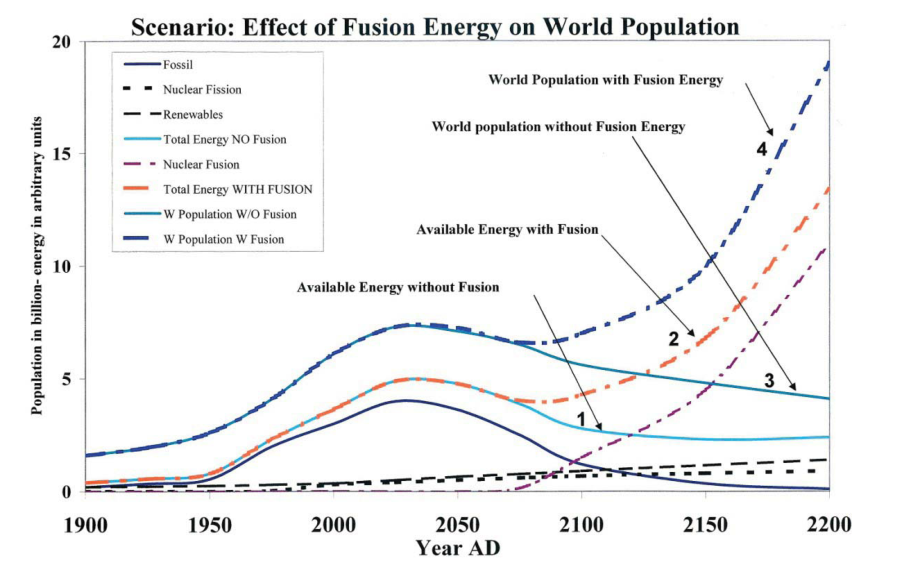
\includegraphics[width=\textwidth]{pic/n.png}
		\caption{基于人口持续增长的能源消耗图}
		\label{fig:example_img}
	\end{center}
\end{figure}
\par 从此图可以看出,核聚变能源的发展即将到来,总能源开始下降的临界点被认为是在本世纪中叶,此后,人类将不得不应对供应的减少,除非不断增加的短缺被核聚变能源弥补。到了下个世纪,核聚变能源应该能够填补这一空白,让人类文明继续进步和增长。而且由于核聚变能源的发展是一个复杂的技术任务可能会有几十年的能源短缺,这将严重影响图中的能源消费。这种能源停滞期和相应的世界人口停滞期即使在核聚变能源的发展和采用的情况下也是不可避免的。在没有核聚变能源的情况下,在此图情形下,世界人口下降到50亿以下,也就意味着人类文明的倒退。因此,为了人类以后文明的发展,核聚变能源的开发和使用是必要的。